\section{Rear: Rear Exocentric Augmented Reality}
\label{sec:rear}

\lstset{language=C}

\subsection{A short introduction to OpenGL}

OpenGL is designed as a software interface to the graphics hardware on your computer. It defines a platform-independent API;
the API is then implemented in software and/or hardware for various machine architectures. The advantage is that OpenGL programs
are easily portable to a variety of computers.
\newline OpenGL provides basic commands to support rendering. In particular, OpenGL doesn't provide functionality to support
windows or user interaction (like keyboard presses or mouse actions); these features are provided by a separate library called
GLUT (the OpenGL Utility Toolkit). GLUT also provides some higher-level features, such as more complex geometrical objects.
\newline OpenGL is a state machine, which means that you specify various states or modes which remain in effect until changed.
Each command that is executed is carried out within the current state. States include things like the current window (where
drawing will appear), color, viewing and projection matrices, drawing modes, positions and characteristics of lights,
materials, and features. These elements will not be introduced throughout this document, as they are already explained in
various tutorials \cite{opengl:brieftutorial} o manual books \cite{opengl:redbook}.
\newline Nevertheless, it is important to keep the idea of a "state machine" in mind as you work with OpenGL in order to 
understand the effects of a given command. The current state is not reset when a function starts or ends - the current state
is in effect until something changes it, regardless of where in the program the next thing is. 

\subsection{Setting up a texture}
\subsection{Lighting in OpenGL}
\subsection{Perspective in OpenGL}

Perspective in OpenGL can be something very trick to work with. It all starts from the definition of 'frustum', as the portion
of space seen from the point of view (see \cite{wiki:frustum} for further information). To define the frustum we use the function
named 'gluPerspective' \cite{opengl:gluPerspective}, which takes four parameters.
\newline The first parameter indicates the FOV (e.g. Field Of View) along the Y axis, in deegres: the chosen value is 60. The
second one expresses ratio between actual width and height, in our case 624/442. The last two parameters specify the distance from
the viewer to the near clipping plane and to the far one, according to the frustum definition.
\newline By using two close values for the far and near clipping planes distance the application will not be able to display 3d
objects, unless the point of view is relatively close to them. If we want to be able to see 3d objects as they are moving away
from the point of view, we need to increase the difference between the last two parameters of the 'gluPerspective' function. In
our case the chosen values are 0.001 and 100000 (its ratio is equal to 10exp8).
\newline The 'gluPerspective' function affects the GL PROJECTION function, previously selected by changing matrix mode. Finally,
in order to set our point of view, we must change matrix again, this time to work with the GL MODELVIEW matrix. The function named
'gluLookAt' allows to set the point of view, with its coordinates, the coordinates of the point to look at and its orientation.
See \cite{opengl:gluLookAt} for further details.

\begin{lstlisting}

  /* define the projection transformation */
  glMatrixMode(GL_PROJECTION);
  glLoadIdentity();
  gluPerspective(60, 624/442, 0.001, 100000);
  
  /* define the viewing transformation */
  glMatrixMode(GL_MODELVIEW);
  glLoadIdentity();
  gluLookAt(0.0, 0.0, 10.0,
            0.0, 0.0, 0.0,
            0.0, 1.0, 0.0);

\end{lstlisting}

To better understand these methods we recommend reading OpenGL manual.

\subsection{The Robot class}

The robot class, present in Filippo Privitera's simulator \cite{privitera}, has been simplified and then introduced in
exocentric vision control code. In this chapter we will exam the main differences.
\newline Both classes represent the 3morduc robot in openGL world. This means that the robot class offers, among others, a
method with the purpose of drawing itself, called by the OpenGL framework when it is necessary. The operation of drawing is
completed thanks to other two methods, able to draw the elementary part of the robot (e.g. cylinders and disks).
\newline There are not considerable different between the tho drawing method implantation. The main one is that in the new method,
before starting drawing, the model-view matrix is copied in order to restore it at the end of the process. In these way we
do not affect the model-view matrix status by drawing the robot.
\newline The robot class, after the refactoring process, loses many of its public attributes and methods, so in the
exocentric vision control it is much more simple than the original one. First of all, the new class does not contain either
attributes to store the actual speed vector component, or a chronometer object to count the time, or information about wheels
encoder. This information was stored in the simulator robot class to calculate the position of the robot after a movement,
but since we retrieve the position directly from the simulator these fields are now useless. 
\newline The unique attribute (changed from public to private, in the new version) which survives the refactory - along with the
triple values indicating coordinate on x axis, coordinate on y axis and rotation - is named 'radius'. 'radius' is a float
attribute, which stores the value of the radius for the tree cylinders which make up the robot. See figure
\ref{fig:3morduc_opengl} for a better understanding.


\begin{figure}[!h]
  \begin{center}
    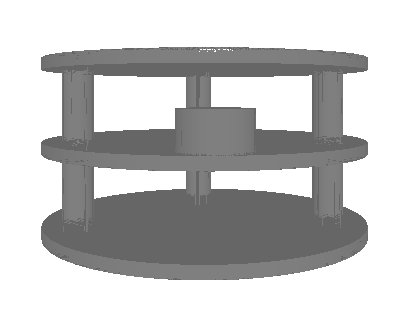
\includegraphics[width=200pt]{img/3morduc_opengl}  %robot pic
    \caption{The 3morduc robotic platform drawn in OpenGL}
    \label{fig:3morduc_opengl}
  \end{center}
\end{figure}


The default 'radius' value is 4, but it can be customized by the user: by increasing it the robot will be 
displayed larger and larger on the screen, and viceversa.
\newline All the attributes are private in the new robot class, so a method to get each one value is declared.
\newline Most of the previous public methods have been removed too. The constructor method, for instance, is present with one
only definition and default parameters, instead of declaring it twice (with parameters and without). The methods to set
linear and angular velocity are not present anymore, for the reason explained above; those to increment the collisions number are
actually disabled because, at this development stage, the exocentric vision control does not face the collision problem.
Anyway, it is supposed to cope with collision in the future version.
\newline Besides, the method used by Privitera's simulator to read the robot initial position from file has been removed, since for
the exocentric vision system robot always starts from fixed coordinates and rotation.
\newline Finally, the method named with the signature 'void move()' has been changed in 'void Place(float x, float y, float theta)',
in order to set the x and y coordinate and the rotation of the robot. We remind that in the previous version these attributes
were public, so there were no need to pass them as parameters function.
